\input header.tex

\title{課題案}
\subtitle{数学・物理をプログラミングで考える}
\author{椎名}
\institute{田浦研究室 TA}
\date{\the\year.\the\month.\the\day}

\begin{document}

\begin{frame}[noframenumbering,plain]
  \titlepage
\end{frame}

\begin{frame}{粒子法による流体シミュレーション (1)}
  ナビエ・ストークス方程式
  \[
    \frac{\partial \bm{v}}{\partial t} + (\bm{v} \cdot \nabla)\bm{v} = - \frac{1}{\rho}\nabla p + \nu \nabla^2\bm{v} + \bm{g}
  \]
  を数値的に解く。

  \bigskip
  この複雑な微分方程式をどう解くか?
  \begin{itemize}
    \item 格子法
    \item 粒子法
    \item ... etc
  \end{itemize}
\end{frame}

\begin{frame}{粒子法による流体シミュレーション (2)}
  \begin{block}{粒子法}
    流体を粒子の集合としてモデル化し、粒子間の相互作用を考えることによって流体のシミュレーションを行う手法
  \end{block}
  粒子法の中でも何種類かあり、下は\structure{SPH法}を用いてシミュレーションしたもの
  \begin{figure}
    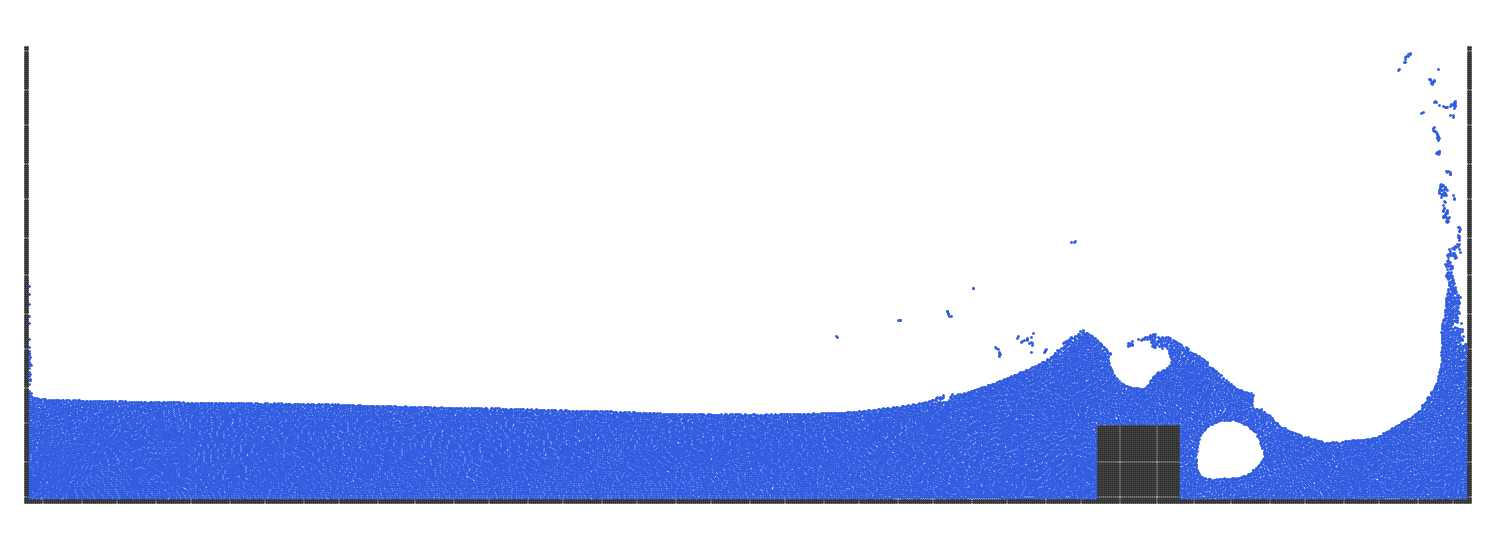
\includegraphics[width=0.6\hsize]{images/dambreaking.png}
  \end{figure}
\end{frame}

\end{document}
